\section{Signature for Sequential Circuit}
In this section, I discussed the signature for two sequential circuits, i.e., 3-bit counter and FIR filter.
\subsection{3-bit Counter}

Figure~\ref{fig:matlab} shows the 3-bit counter in MATALB Simulink. I have derived the signature by stuck-at-fault model to all different possible nodes. Table~\ref{s@1-O0}  shows the signature values if the node B0 stuck at "1." Similarly, I have derived the signatures of all the nodes.

\begin{figure}[tb!]
 \centering
  \captionsetup{justification=centering}    
   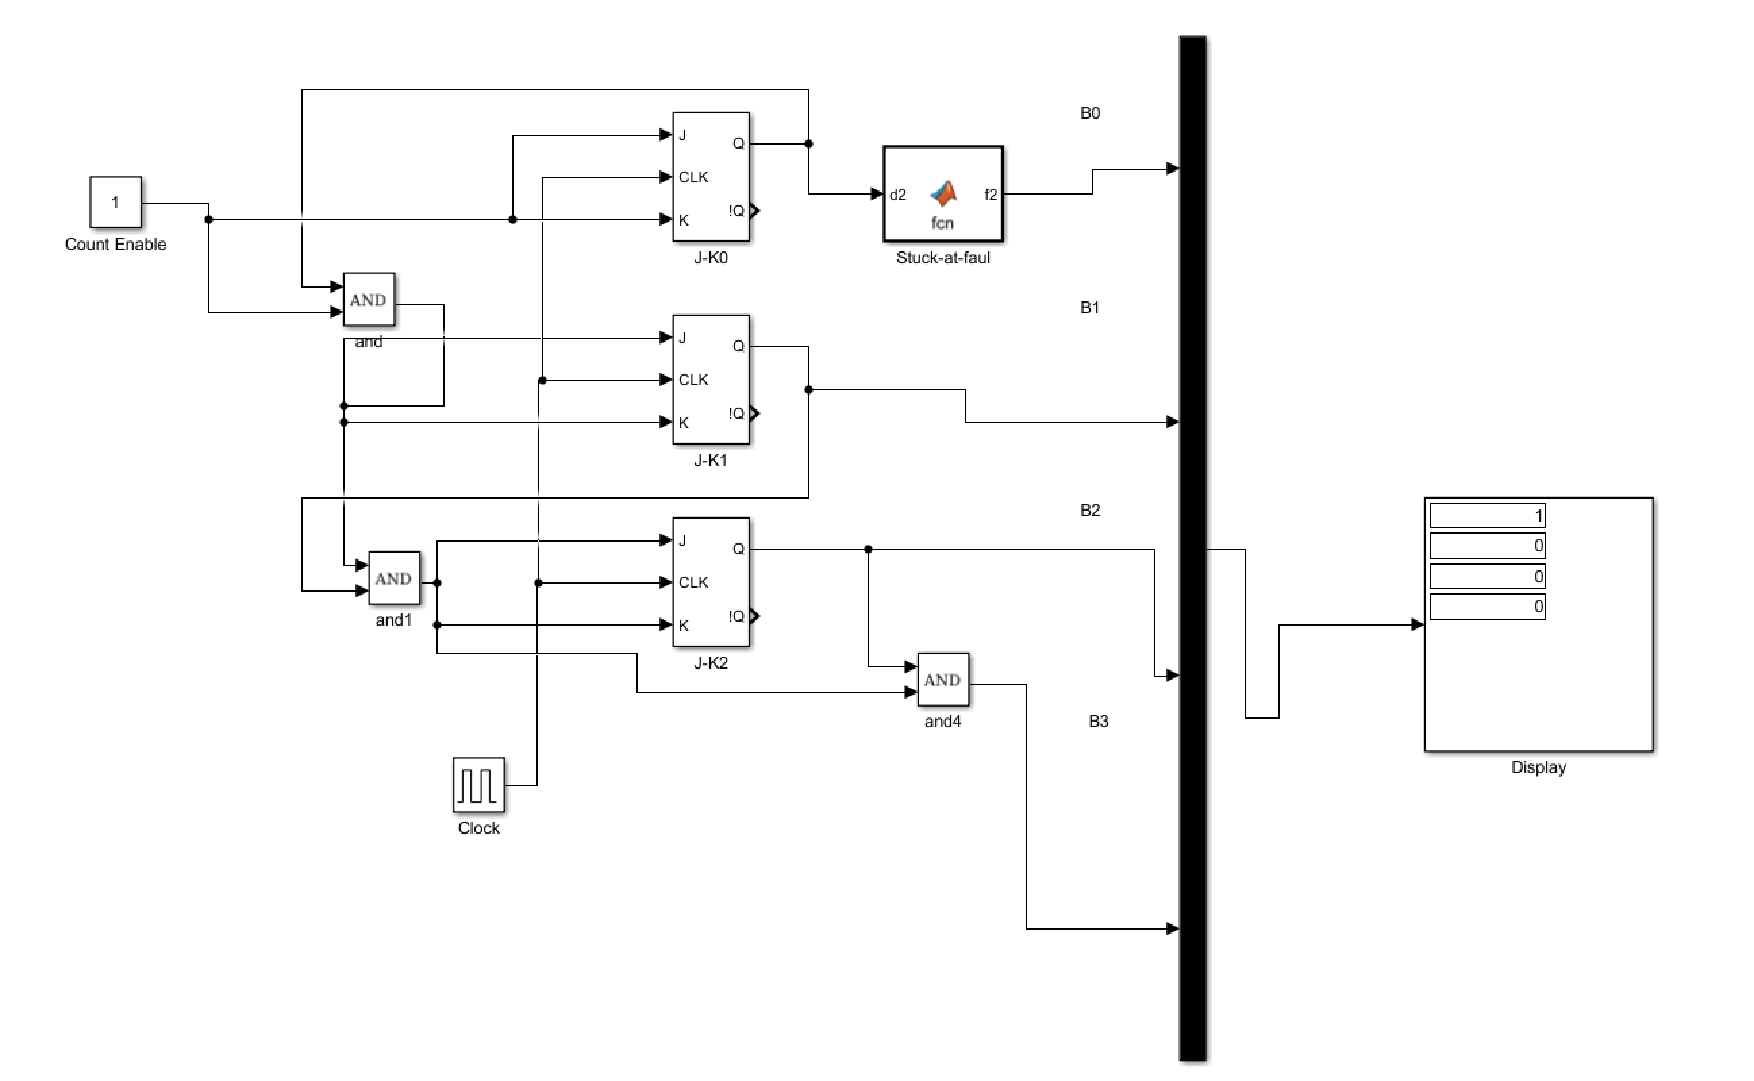
\includegraphics[scale=0.4]{Figures/matlab-counter.pdf}
   \caption{3-bit counter in MATALB.}
\label{fig:matlab}
\end{figure}

\begin{table}[tb!]
\center
\caption{Stuck-at-1$\rightarrow O_0$.}
\label{s@1-O0}
\begin{tabular}{|c | c| c | c| } 
 \hline
 \rowcolor{lightgray}
Faulty Value (Binary) & Faulty Value & Original Value & Arithmetic Signature   \\ 
\hline
 
 
 001& 1 &0 & -1  \\
 \hline
 011 & 3 & 1 & -2 \\ 
 \hline
 
 101 & 5 & 2 & -3 \\
 \hline
 111& 7& 3& -4 \\
 \hline
 001 & 1  &  4& 3 \\
 \hline
 011 & 3 & 5 &2  \\
 \hline
 101 & 5 & 6 & 1 \\
 \hline
 111 & 7 & 7 & 0 \\
 \hline
 
 
\end{tabular}
\end{table}

\section{Signature for FIR Filter}


In this example I have applied stuck-at-fault to different nodes in the FIR filter as shown in Figure~\ref{fig:filter} and find their respective Signatures.



\begin{figure}[tb!]
 \centering
  \captionsetup{justification=centering}    
   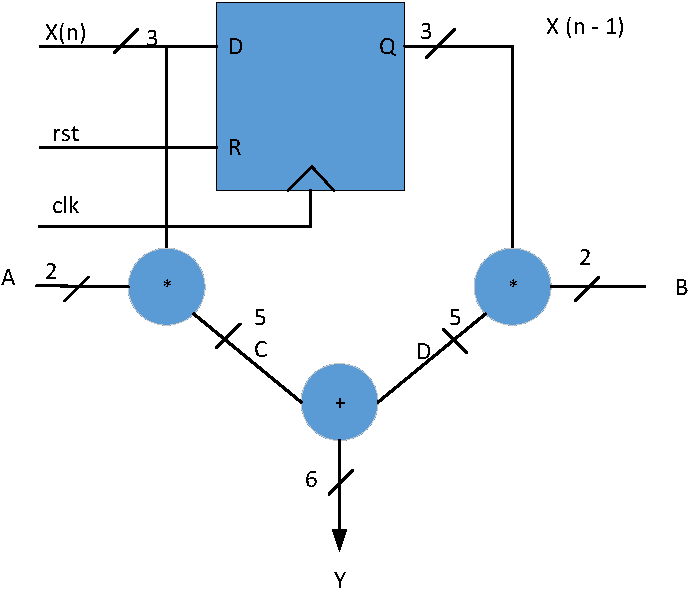
\includegraphics[scale=0.7]{Figures/FIR.pdf}
   \caption{FIR Filter.}
\label{fig:filter}
\end{figure}





\begin{table}[tb!]
\center
\caption{Stuck-at-0$\rightarrow Y_0$}
\label{s@1-O0}
\begin{tabular}{|c | c| c | c| c |} 
 \hline
 \rowcolor{lightgray}
Decimal Golden & Binary & Stuck@0$\rightarrow Y_0$ & Decimal Faulty & Arithmetic Signature   \\ 
\hline
 
 
 0 & 000000 & 000000 & 0 & 0  \\
 \hline

 1 & 000001 & 000000 & 0 & 1 \\
 \hline
 
 6 & 000110 & 000110 & 6 & 0 \\
 \hline
 15 & 001111 & 001110 & 14 & 1 \\
 \hline
 14 & 001110 & 001110 & 14 & 0 \\
 \hline
 27 & 011011 & 011010 & 26 & 1 \\
 \hline
 11 & 001011 & 001010 & 10 & 1 \\
 \hline
 0 & 000000 & 000000 & 0 & 0 \\
 \hline
 0 & 000000 & 000000 & 0 & 0 \\
 \hline
 11 & 001011 & 001010 & 10 & 1 \\
 \hline
 18 & 010010 & 010010 & 18 & 0 \\
 \hline
 
 21 & 010101 & 010100 & 20 & 1 \\
 \hline
 10 & 001010 & 001010 & 10 & 0 \\
 \hline
 9 & 001001& 001000 & 8 & 1 \\
 \hline
 1 & 000001 & 000000 & 0 & 1 \\
 \hline
 0 & 000000 & 000000 & 0 & 0 \\
 \hline




 
 
\end{tabular}
\end{table}



















